\chapter{Maximum Flow}
\section{Flow}
Suppose we are given a directed graph $G=(V,E)$ with a source vertex $s$ and a target vertex $t$. And additionally for every edge $e\in E$ we are given a number $c_e\in \bbZ_0$ which is called the capacity of the edge.
\begin{Definition}{Flow}{}
	An $s-t$ flow is a function $f:E\to\bbR_0$ which satisfies the following:\begin{enumerate}[label=\protect\circled{\small\arabic*}]
		\item $\forall\ e\in E$, $f(e)\leq c_e$
		\item $\forall\ v\in V\setminus\{s,t\}$, $\sum\limits_{e\in \textit{in}(v)}f(e)=\sum\limits_{e\in \textit{out}(v)}f(e)$
	\end{enumerate}
Also the value of a flow $f$ is denoted by $|f|\coloneqq \sum\limits_{e\in \textit{out}(s)}f(e)$.
\end{Definition}Before proceeding into the setup and the problem first we will assume some things
\begin{assumption*} 
	\begin{itemize}
		\item $\textit{in}(s)=\emptyset$ i.e. there is no edge into $s$.
		\item $\textit{out}(t)=\emptyset$ i.e. there is no edge out of $t$.
		\item There are no parallel edges
	\end{itemize}
\end{assumption*}
\begin{lemma}{}{}
	For any flow $f$, $|f|=\sum\limits_{e\in \textit{in}(t)}f(e)$
\end{lemma}
\begin{proof}
	We have for every edge $e\in E$, $\exs\ v\in V$ such that $e\in \textit{in}(v)$ and $\exs\ u\in V$ such that $e\in \textit{out}(u)$. Hence we get $$\sum_{e\in E}f(e)=\sum_{v\in V}\sum_{e\in\textit{in}(v)}f(e)=\sum_{v\in V}\sum){e\in\textit{out}(v)}f(e)\implies \sum_{v\in V}\lt[\sum_{e\in\textit{in}(v)}f(e)-\sum_{e\in\textit{out}(v)}f(e)\rt]=0$$
	Now we know $\forall\ v\in V\setminus\{s,t\}$. $\sum\limits_{e\in\textit{in}(v)}f(e)=\sum\limits_{e\in\textit{out}(v)}f(e)$. Therefore we get $$ \sum_{v\in V}\lt[\sum_{e\in\textit{in}(v)}f(e)-\sum_{e\in\textit{out}(v)}f(e)\rt]=0\implies \sum_{v\in \{s,t\}}\lt[\sum_{e\in\textit{in}(v)}f(e)-\sum_{e\in\textit{out}(v)}f(e)\rt]=0\implies \sum\limits_{e\in \textit{out}(s)}f(e)-\sum\limits_{e\in \textit{in}(t)}f(e)$$Hence we have $|f|=\sum\limits_{e\in \textit{in}(t)}f(e)$.
\end{proof}

%Now the problem we will study is to given such a graph find a flow which maximizes the value.
\begin{algoprob}
	\problemtitle{Max Flow}
	\probleminput{A directed graph $G=(V,E)$ with source vertex $s$ and target vertex $t$ and for all edge $e\in E$ capacity of the edge $c_e\in\bbZ_+$}
	\problemquestion{Given such a graph and its capacities find an $s-t$ flow which has the maximum value}
\end{algoprob}

\begin{Example}{}{}
	Consider the following directed graph with capacities: $V=\{s,t,u,v\},\quad c_{s,u}=2,c_{s,v}=c_{u,t}=c_{v,t}=c_{u,v}=1$. Firstly the following function: $f':f'(s,u)=2=f(u,t)$. It is not a flow since $f(u,t)=2>1=c_{u,t}$. Now we define three different flow functions:
	\begin{center}
	\begin{tikzpicture}[scale=1.5]
	% Draw vertices with circles around them
\begin{scope}[shift={(-5,0)}]
		\node[draw, circle] (A) at (0, 0) {$s$};
	\node[draw, circle] (B) at (2, 1) {$u$};
	\node[draw, circle] (C) at (2, -1) {$v$};
	\node[draw, circle] (D) at (4, 0) {$t$};
	
	% Draw directed edges with values and reduced bends
	\draw[,-latex, bend left=15] (A) to node[below] {2} (B);
	\draw[,-latex, bend left=15] (B) to node[below] {1} (D);
	\draw[,-latex] (B) -- node[left] {1} (C);
	\draw[,-latex, bend right=15] (A) to node[above] {1} (C);
	\draw[,-latex, bend right=15] (C) to node[above] {1} (D);
	
	
    % Draw a single continuous red path from A to B to C to D
\draw[red!80!black, thick, ,-latex, rounded corners=5pt] 
($(A) + (0.1, 0.4)$) to [bend left=15] node[above] {1} ($(B) + (-0.4, 0.2)$) 
-- node[left] {1} ($(C) + (-0.4, -0.35)$) to [bend right=18] node[below] {1}($(D) + (-0.2, -0.5)$);
\draw[blue, thick, ,-latex, rounded corners=12pt, bend left=70] ($(A) + (0, 0.6)$) to node[above, xshift=-2.5cm, yshift=-0.85cm]{1} node[above, xshift=2.5cm, yshift=-0.85cm] {1}($(D) + (-0, 0.6)$);
\draw[blue, thick, ,-latex, rounded corners=12pt, bend right=70] ($(A) + (0, -0.6)$) to node[below, xshift=-2.5cm, yshift=0.85cm]{1} node[below, xshift=2.5cm, yshift=0.85cm]{1} ($(D) + (0, -0.6)$);
\draw[green!60!black, thick, rounded corners=12pt, bend left=23] ($(A) + (0.5, 0)$) to node[below]{2} ($(B) + (0.2,-0.39)$);
\draw[green!60!black, thick,,-latex, rounded corners=12pt, bend left=17]  ($(B) + (0.2,-0.39)$)  to node[below]{1} ($(D) + (-0.5,0)$)  ;
\draw[green!60!black, thick, rounded corners=5pt,-latex]  ($(B) + (0.2,-0.39)$)  to  node[right]{1}($(C) + (0.2,0.35)$)  to [bend right=23] node[above]{1} ($(D) + (-0.5,0)$);

\end{scope}
\begin{scope}[shift={(1.5,0)}]
	\draw (1,0) node[text width=8cm]{\begin{itemize}
			\item \textcolor{red!80!black}{$f\colon f(s,u)=f(u,v)=f(v,t)=1$ and otherwise $0$. Therefore $|f|=1$}
			\item \textcolor{blue}{$g\colon g(s,u)=g(u,t)=1$, $g(s,v)=g(v,t)=1$ and otherwise $0$. Therefore $|g|=2$}
			\item \textcolor{green!50!black}{$h\colon h(s,u)=2$, $h(u,t)=h(u,v)=h(v,t)=1$ and otherwise $0$. Therefore $|h|=2$}
	\end{itemize}\vspace*{5mm}

Notice here $g$ and $h$ has the maximum flow value.};
\end{scope}
\end{tikzpicture}
\end{center}
\end{Example}


\section{Ford-Fulkerson Algorithm}
\begin{Definition}{Residual Graph}{}
	Given a directed graph $G=(V,E)$ and capacities $C_e$ for all $e\in E$ and an $s-t$ flow $f$ the residual graph $G_f=(V,E_f)$ has the edges with the following properties:
	\begin{enumerate}[label=\protect\circled{\arabic*}]
		\item If $(u,v)\in E$ and $f(u,v)>0$  then $(v,u)\in E_f$ and $c_{v,u}^f=f(u,v)$. Such an edge is called a \textit{backward} edge.
		\item If $(u,v)\in E$ and $f(u,v)<c_{u,v}$ then $(u,v)\in E_f$ and $c_{u,v}^f=c_{u,v}-f(u,v)$. It is called \textit{forward} edge.
	\end{enumerate}
\end{Definition}

\begin{algorithm}\label{ford-fulkerson}
\DontPrintSemicolon
\SetKwComment{Comment}{//}{}
\KwIn{Directed graph $G=(V,E)$, source $s$, target $t$ and edge capacities $C_e$ for all $e\in E$}
\KwOut{Flow $f$ with maximum value}
\Begin{
	\For{$e\in E$}{$f(e)=0$}
	\While{$\exs\ s\rightsquigarrow t$ path $P$ in $G_f$}{
	$\dl\longleftarrow \min\limits_{e\in P}\{c_e^f\}$
	\For{$e=(u,v)\in P$}{
	\If{$e$ is Forward Edge}{$f(u,v)\longleftarrow f(u,v)+\dl$}
	\Else{$f(u,v)\longleftarrow f(v,u)-\dl$}
}
}	
}
\caption{\prb{Ford-Fulkerson}}
\end{algorithm}
We call one iteration of the While loop at line 4 \textit{Flow Augmentation}.
%\begin{note}
%	In each flow augmentation some edge will disappear. This is because the 
%\end{note}
\begin{lemma}{}{flowaugment}
	At any iteration the $f'$ obtained after the flow augmentation of the flow $f$ is a valid flow
\end{lemma}
\begin{proof}
	At any iteration  let $P$ be the path from $s\rightsquigarrow t$ and $\dl=\min\limits_{e\in P}c_f(e)$. Let $f'$ be the new function such that for each $(u,v)\in P$ if $(u,v)$ is forward edge in $G_f$ then $f'(u,v)=f(u,v)+\dl$ and if $(u,v)$ is backward edge in $G_f$ then $f'(v,u)=f(v,u)-\dl$ and for other edges $e\in E\setminus P$, $f'(e)=f(e)$. 
	
		Now since $\dl=\min\limits_{e\in P}c_f(e)$, $c_f(e)\geq \dl$ for all $e\in P$. Hence if $(u,v)$ is backward edge then $(v,u)\in E$ and $c_f(u,v)=f(u,v)$. Hence $f'(v,u)=f(v,u)-\dl\geq 0$. Therefore for all $e\in E$, $f'(e)\geq 0$. 
	
	Now first we will show $f'(e)\leq c_e$ for all $e\in E$. If $(u,v)\in P$ is a forward edge then $(u,v)\in E$ and $c_f(u,v)=c_{u,v}f(u,v)$. Therefore $f'(u,v)=f(u,v)+\dl\leq f(u,v)+c_{u,v}-f(u,v)=c_{u,v}$. Now if $(u,v)\in P$ is a backward edge then $(v,u)\in E$ and $c_f(u,v)=f(u,v)$. Therefore $f'(u,v)=f(u,v)-\dl\leq f(u,v)\leq c_{u,v}$. For other edges $e\in E\setminus P$, $f'(e)=f(u)\leq c_e$. Therefore $f'(e)\leq c_e$ for all $e\in E$
	
	Now we will prove for all $v\in V\setminus\{s,t\}$, $\sum\limits_{e\in \textit{in}(v)}f'(e)=\sum\limits_{e\in\textit{out}(v)}f'(e)$. If $v$ is not in the path $P$ in $G_f$ then, $f'(e)=f(e)$ for all edges $e\in \textit{in}(v)\cup \textit{out}(v)$. Hence the condition is satisfied for such vertices. Suppose $v$ is in the path $P$. Then there are two edges $e_1$ and $e_2$ in $P$ which are incident on $e$. If both are forward edges or both are backward edges then one of them is in $\textit{in}(v)$ and other one is in $\textit{out}(v)$. WLOG suppose $e_1\in \textit{in}(v)$ and $e_2\in\textit{out}(v)$ we have $$\sum\limits_{e\in \textit{in}(v)}f'(e)=\sum\limits_{e\in \textit{in}(v)\setminus\{e_1\}}f(e)+f(e_1)\pm \dl=\sum\limits_{e\in\textit{out}(v)\setminus \{e_2\}}f(e)+f(e_2)\pm \dl=\sum\limits_{e\in\textit{out}(v)}f'(e)$$If one of $e_1$, $e_2$ forward edge and other one is backward edge then either $e_1,e_2\in \textit{in}(v)$ (when $e_1$ is forward and $e_2$ is backward) or $e_1,e_2\in \textit{out}(v)$ (when $e_1$ is backward and $e_2$ is forward). Now if $e_1,e_2\in \textit{in}(v)$, $f'(e_1)+f'(e_2)=f(e_1)+\dl+f(e_2)-\dl=f(e_1)+f(e_2)$ and if $e_1,e_2\in\textit{out}(v)$ then $f'(e_1)+f'(e_2)=f(e_1)-\dl+f'(e_2)+\dl=f(e_1)+f(e_2)$. Hence $$\sum\limits_{e\in \textit{in}(v)}f'(e)=\sum\limits_{e\in \textit{in}(v)}f(e)=\sum\limits_{e\in\textit{out}(v)}f(e)=\sum\limits_{e\in\textit{out}(v)}f'(e)$$ Hence $f'$ is a valid flow. 
\end{proof}

\begin{lemma}{}{flowaugment-flowvalue}
	At any iteration Given $G_f$ if the flow, $f'$ obtained after flow augmentation of $f$ by $\dl$ then $$|f'|=|f|+\dl$$
\end{lemma}
\begin{proof}
	Since we augment flow along an $s\rightsquigarrow t$ path, the first edge of the path is always in \textit{out}$(s)$. Let the first edge is $e=(s,u)$. Now $e$ has to be a forward edge because otherwise $(u,s)\in E$ and then there is an incoming edge in $G$ which is not possible. Hence $$|f'|=\sum\limits_{e\in \textit{out}(s)}f'(e)=\sum_{e\in \textit{out}(s)\setminus\{e\}}f(e)+f'(e)=\sum_{e\in \textit{out}(s)\setminus\{e\}}f(e)+f(e)+\dl=\sum_{e\in\textit{out}(s)}f(e)+\dl=|f|+\dl$$Hence we have the lemma.
\end{proof}
\begin{lemma}{}{}
	At every iteration of the Ford-Fulkerson Algorithm the flow values and the residual capacities of the residual graph are non-negative integers.
\end{lemma}
\begin{proof}
	Initial flow and the residual capacities are non-negative integers. Let till $i^{th}$ iteration the flow values and the residual capacities were non-negative integers. Let the flow after $i^{th}$ iteration was $f$. Hence $\forall\ e\in E$, $f(e)\in \bbZ_0$. Therefore in the $G_f$ for all $e\in E_f$, $c_f(e)\in\bbZ_0$. Hence $\dl\in\bbZ_0$. Therefore $\forall\ e\in E$, $f'(e)\in\bbZ_0$. And therefore for all $e\in E_{f'}$ where $G_{f'}$ is the residual graph of the flow $f'$, $c_{f'}(e)\in\bbZ_0$. Hence by mathematical induction the lemma follows.
\end{proof}
At any iteration let $P$ be the path from $s\rightsquigarrow t$. Then for all $e\in P$, $c_f(e)>0$. Therefore $\dl=\min\limits_{e\in P}c_f(e)\geq 1$. Therefore the algorithm must stop in at most $\sum\limits_{e\in \textit{out}(s)}c_e$ since we can have the value of a flow to be at max the value of the sum of capacities of edges in \textit{out}$(s)$ and therefore we can increase the flow at max that many times.
\begin{lemma}{}{maxflownopath}
	If $f$ is a max flow then there is no $s\rightsquigarrow t$ path in $G_f$.
\end{lemma}
\begin{proof}
	Suppose there is an $s\rightsquigarrow t$ path $P$ in $G_f$. We will show that then $f$ is not a max flow following the algorithm. Then $\forall\ e\in P$, $c_f(e)>0$. Hence $\dl=\min\limits_{e\in P}c_f(e)\geq 1$. Now after the flow augmentation process of $f$ by $\dl$ we get a new valid flow $f'$ by \lmref{flowaugment} and by \lmref{flowaugment-flowvalue} we have $|f'|=|f|+\dl>||f|$. Hence $f$ is not a maximum flow. Hence contradiction. Therefore there is no $s\rightsquigarrow t$ path in $G_f$.
\end{proof}
\subsection{Max Flow Min Cut}
\dfn{Cut Set}{For a graph $G=(V,E)$ and a subset $A\subseteq V$, the cut $(A,V\setminus A)$ is  a bipartition of $V$ where  the edges $E_A$ of the graph $G_A=(A,V\setminus A, E_A)$ is the set  $E_A= E\cap (A\times (V\setminus A))$.\parinn
	
	Now if $s,t$ are two vertices of $G$ then an $s-t$ \textit{Cut} $(A,V\setminus A)$ is a cut such that $s\in A$ and $t\in V\setminus A$.}
 Now we define for a cut $(A,V\setminus A)$ the \textit{Capacity of the Cut} $(A,V\setminus A)=\sum\limits_{e\in E_A}c_e$. For an $s-t$ cut $(A,V\setminus A)$ we denote the capacity of the cut by $\textit{cap}(A)$ A \textit{Min $s-t$ Cut} is a $s-t$ cut of minimum capacity. Then we have the following relation between cut and flow.
 \begin{lemma}{}{flowlessthancapacity}
 	Given a graph $G=(V,E)$, $s$, $t$, $c_e\in\bbZ_0$ for all $e\in E$ for any flow $f$ and a $s-t$ cut $(A,V\setminus A)$ $$|f|\leq \textit{cap}(A)$$
 \end{lemma}
\begin{proof}
	Given $f$ and the $s-t$ cut $(A,V\setminus A)$ we have \begin{align*}
		|f| & = \sum_{e\in\textit{out$(s)$}}f(e)\\
		& = \sum_{v\in A}\lt[ \sum_{e\in\textit{out(v)}}f(e)-\sum_{e\in \textit{in$(v)$}}f(e)  \rt]\\
		& = \sum_{\substack{e=(u,v),\\ u\in A,v\notin A}}f(e) -\sum_{\substack{e=(u,v),\\ u\notin A,v\in A}}f(e) & [\text{Edges for both endpoints in $A$ are canceled out}]\\
		&=\sum_{e\in \textit{out$(A)$}}f(e)-\sum_{e\in \textit{in}(A)}f(e)\\
		& \leq \sum_{e\in \textit{out$(A)$}}f(e)\leq \sum_{e\in \textit{out$(A)$}}c_e=\textit{cap}(A)
	\end{align*}
Hence we have the lemma.
\end{proof}
Having this lemma we have have for any flow $f$ and $s-t$ cut $(A,V\setminus A)$ we have $$|f|\leq \textit{cap$(A)$}\implies \max\limits_f|f|\leq\min\limits_{s-t\textit{ cut $(A,V\setminus A$)}}\textit{cap$(A)$}$$So we have the following theorem that the value of maximum flow is equal to the capacity of minimum cut.
 \begin{Theorem}{Max Flow Min Cut}{}
 	Given a graph $G=(V,E)$, $s$, $t$, $c_e\in\bbZ_0$ for all $e\in E$. Then \tfae\begin{enumerate}[label=(\arabic*)]
 		\item $f$ is a maximum flow.
 		\item There is no $s\rightsquigarrow t$ path in $G_f$
 		\item There exists an $s-t$ cut of capacity $|f|$
 	\end{enumerate}
 \end{Theorem}
\begin{proof}
	\begin{itemize}[leftmargin=2cm]
		\item[(1)$\implies$(2):] This is by \lmref{maxflownopath}.
		\item[(2)$\implies$(3):] We are given a flow $f$ such that there is no $s\rightsquigarrow t$ path in $G_f$. We will construct a $s-t$ cut which has the capacity $|f|$. Now take $A$ to be all the vertices reachable from $s$ in $G_f$. This is a valid $s-t$ cut since $s\in A$ and as there is no $s\rightsquigarrow t$ path in $G_f$, $t\notin A$. Now $$|f|=\sum_{e\in \textit{out$(A)$}}f(e)-\sum_{e\in\textit{in$(A)$}}f(e)$$Now $\forall\ e=(u,v)\in E$ where $u\in A$ and $v\notin A$ we have  $c_{u,v}=f(u,v)\implies c_{u,v}-f(u,v)=0$ since otherwise $c_{u,v}-f(u,v)\neq 0\implies c_{u,v}>f(u,v)\implies (u,v)\in E_f$ and therefore $v$ is reachable from $s$ but $v\notin A$, contradiction. Therefore $(u,v)$ is a backward edge and hence . Now $\forall\ e=(u,v)\in E$ where $u\notin A$ and $v\in A$ we have $f(u,v)=0$ since otherwise   $f(u,v)>0\implies (v,u)\in E_f$ and therefore $u$ is reachable from $s$ but $u\notin A$, contradiction. Hence we have $$|f|=\sum_{e\in \textit{out$(A)$}}f(e)-\sum_{e\in\textit{in$(A)$}}f(e)=\sum_{e\in \textit{out$(A)$}}c_e=\textit{cap}(A)$$
		\item[(3)$\implies$(1):] Now by \lmref{flowlessthancapacity} we have for any flow $f$ and $s-t$ cut $$|f|\leq \textit{cap$(A)$}\implies \max\limits_f|f|\leq\min\limits_{s-t\textit{ cut $(A,V\setminus A$)}}\textit{cap$(A)$}$$Now given $f$ there exists an $s-t$ cut of capacity $|f|$. Hence $f$ is a max flow.
	\end{itemize}
\end{proof}
Hence at the end of the \hyperref[ford-fulkerson]{Ford-Fulkerson Algorithm} let the flow returned by the algorithm is $f$. The algorithm terminates when there is no $s\rightsquigarrow t$ path in $G_f$. Hence by \hyperref[th:maxflowmincut]{Max Flow Min Cut Theorem} we have $f$ is a maximum flow. This completes the analysis of the Ford-Fulkerson Algorithm.

Since the capacities of the edges can be very large we want an algorithm return the maximum flow with running time $\textit{poly}(n,m,\log c_e)$ where $n$ is the number of vertices and $m$ is number of edges and $\log c_e$ basically means number of bits at most needed to represent the capacities. 

But Ford-Fulkerson algorithm takes does not run in \textit{poly}$(n,m,\log c_e)$ instead $\textit{poly}(n,m,c_e)$ as the while loop in the algorithm takes $\textit{poly}(c_e)$ many iterations. For example in the following graph: it takes around 100 steps
\begin{center}
	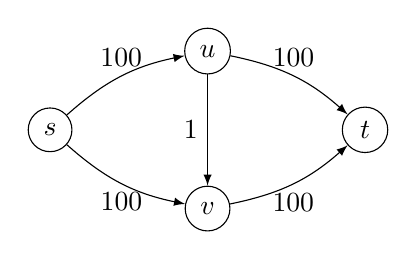
\begin{tikzpicture}
		\node[draw, circle] (A) at (0, 0) {$s$};
		\node[draw, circle] (B) at (2, 1) {$u$};
		\node[draw, circle] (C) at (2, -1) {$v$};
		\node[draw, circle] (D) at (4, 0) {$t$};
		
		% Draw directed edges with values and reduced bends
		\draw[,-latex, bend left=15] (A) to node[above] {100} (B);
		\draw[,-latex, bend left=15] (B) to node[above] {100} (D);
		\draw[,-latex] (B) -- node[left] {1} (C);
		\draw[,-latex, bend right=15] (A) to node[below] {100} (C);
		\draw[,-latex, bend right=15] (C) to node[below] {100} (D);
	\end{tikzpicture}
\end{center}
and in general  Ford-Fulkerson takes $O(|f_{\max}|)$ time. For this reason we will now discuss a modification of the Ford-Fulkerson Algorithm which takes $\textit{poly}(n,m,\log c_e)$ time, Edmonds-Karp Algorithm. 
\subsection{Edmonds-Karp Algorithm}
To get a \textit{poly}$(n,m,\log c_e)$ time algorithm  we will always pick the shortest $s\rightsquigarrow t$  path in the residual graph. This algorithm is known as the Edmonds-Karp Algorithm

Suppose $f_i$ be the total flow after $i^{th}$ iteration. And $G_{f_i}$ be the residual graph with respect $f_i$. Then $f_0(e)=0$ for all $e\in E$ and $G_{f_0}=G$. Also suppose $\textit{dist}_i(v)=$ Shortest $s\rightsquigarrow v$ path distance in the residual graph $G_{f_i}$. Hence $\textit{dist}_i(s)=0$ for all $i$ and $\textit{dist}_i(t)=\infty$ at the end of the algorithm. 
\begin{note}
	In $i^{th}$ iteration of the Ford-Fulkerson Algorithm or Edmonds-Karp Algorithm if $P$ is the $s\rightsquigarrow t$ in the residual graph $G_{f_i}$ where $e=(u,v)\in P$  and $c_{f_i}(u,v)=\dl=\min\limits_{e\in P}c_{f_i}(e)$ then the edge $(u,v)$ is not present in the next residual graph $G_{f_{i+1}}$. Thus at least one edge disappears in each iteration of Ford-Fulkerson or Edmonds-Karp Algorithm.
\end{note}
Now we will prove following two lemmas which will help us to prove that the Edmond-Karp algorithm takes $O(mn)$ iterations. 
\begin{lemma}{}{}
At any iteration $i$, 	$\forall\ v\in V$, $\textit{dist}_i(v)\leq\textit{dist}_{i+1}(v)$
\end{lemma}


\begin{lemma}{}{}
	For any edge $e=(u,v)\in E$ the number of iterations where either $(u,v)$ appears or $(v,u)$ appears is at most $O(n)$ i.e. $$\lt|\lt\{i\colon (u,v)\notin G_{f_i}, (u,v)\in G_{f_{i+1}}\rt\}\rt|+\lt|\lt\{i\colon (v,u)\notin G_{f_i}, (v,u)\in G_{f_{i+1}}\rt\}\rt|=O(n)$$
\end{lemma}
\section{Preflow-Push/Push Relabel Algorithm}